%
% This document contains the chapter about S-parameters.
%
% Copyright (C) 2003, 2004, 2005, 2006 Stefan Jahn <stefan@lkcc.org>
% Copyright (C) 2004, Michael Margraf <Michael.Margraf@alumni.TU-Berlin.DE>
%
% Permission is granted to copy, distribute and/or modify this document
% under the terms of the GNU Free Documentation License, Version 1.1
% or any later version published by the Free Software Foundation.
%

\chapter{Scattering parameters}
%\addcontentsline{toc}{chapter}{Scattering parameters}

\section{Introduction and definition}
%\addcontentsline{toc}{section}{Introduction and definition}

Voltage and current are hard to measure at high frequencies.  Short
and open circuits (used by definitions of most n-port parameters) are
hard to realize at high frequencies.  Therefore, microwave engineers
work with so-called scattering parameters (S parameters), that uses
waves and matched terminations (normally $50 \Omega$).  This procedure
also minimizes reflection problems.

\addvspace{12pt}

A (normalized) wave is defined as ingoing wave $\underline{a}$ or
outgoing wave $\underline{b}$:

\begin{equation}
\underline{a} =
  \underbrace{\dfrac{\underline{u}+\underline{Z}_0\cdot \underline{i}}{2}}_{\underline{U}_{forward}}
  \cdot \dfrac{1}{\sqrt{|\text{Re}\underline{Z}_0)|}}
\qquad\qquad
\underline{b} =
  \underbrace{\dfrac{\underline{u}-\underline{Z}_0^*\cdot \underline{i}}{2}}_{\underline{U}_{backward}}
  \cdot \dfrac{1}{\sqrt{|\text{Re}\underline{Z}_0)|}}
\label{equ:waves}
\end{equation}
where $\underline{u}$ is (effective) voltage, $\underline{i}$
(effective) current flowing into the device and $\underline{Z}_0$ reference
impedance. The waves are related to power in the following way.
\begin{equation}
P = \left( |\underline{a}|^2 - |\underline{b}|^2 \right)
\end{equation}
Sometimes waves are defined with peak voltages and peak currents.
The only difference that appears then is the relation to power:
\begin{equation}
P = \frac{1}{2}\cdot \left( |\underline{a}|^2 - |\underline{b}|^2 \right)
\end{equation}
Now, characterizing an n-port is straight-forward:
\begin{equation}
\begin{pmatrix}
\underline{b}_1\\
\vdots\\
\underline{b}_n\\
\end{pmatrix}
=
\begin{pmatrix}
\underline{S}_{11} & \ldots & \underline{S}_{1n}\\
\vdots & \ddots & \vdots\\
\underline{S}_{n1} & \ldots & \underline{S}_{nn}\\
\end{pmatrix}
\cdot
\begin{pmatrix}
\underline{a}_1\\
\vdots\\
\underline{a}_n\\
\end{pmatrix}
\end{equation}

One final note: The reference impedance $\underline{Z}_0$ can be
arbitrary chosen. It normally is real, and there is no urgent
reason to use a complex one. The definitions in equation
\ref{equ:waves}, however, are made form complex impedances. These
ones stem from \cite{Kurokawa}, where they are named "power waves".
These power waves are a useful way to define waves with complex
reference impedances, but they differ from the waves introduced
in the following chapter. For real reference impedances both
definitions equal each other.


\section{Waves on Transmission Lines}

This section should derive the existence of the voltage and current
waves on a transmission line.  This way, it also proofs that the
definitions from the last section make sense.

\begin{figure}[ht]
\begin{center}
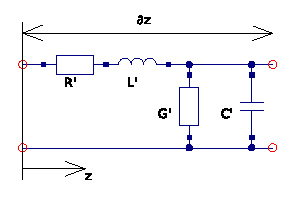
\includegraphics[width=6cm]{TLpiece}
\end{center}
\caption{Infinite short piece of transmission line}
\label{fig:tlpiece}
\end{figure}
\FloatBarrier

Figure \ref{fig:tlpiece} shows the equivalent circuit of an infinite
short piece of an arbitrary transmission line.  The names of the
components all carry a single quotation mark which indicates a per-length
quantity. Thus, the units are ohms/m for $R'$, henry/m for $L'$,
siemens/m for $G'$ and farad/m for $C'$. Writing down the change of
voltage and current across a piece with length $\partial z$ results
in the transmission line equations.

\begin{equation}
\dfrac{\partial u}{\partial z} = - R' \cdot i(z) - L' \cdot \dfrac{\partial i}{\partial t}
\end{equation}
\begin{equation}
\dfrac{\partial i}{\partial z} = - G' \cdot u(z) - C' \cdot \dfrac{\partial u}{\partial t}
\end{equation}

Transforming these equations into frequency domain leads to:

\begin{equation}
\label{eqn:tlf1}
\dfrac{\partial\underline{U}}{\partial z} = -\underline{I}(z)\cdot (R' + j\omega L')
\end{equation}
\begin{equation}
\label{eqn:tlf2}
\dfrac{\partial\underline{I}}{\partial z} = -\underline{U}(z)\cdot (G' + j\omega C')
\end{equation}

Taking equation \ref{eqn:tlf2} and setting it into the first derivative of
equation \ref{eqn:tlf1} creates the wave equation:

\begin{equation}
\dfrac{\partial^2\underline{U}}{\partial z^2} = \underline{\gamma}^2 \cdot \underline{U}
\end{equation}
with $\underline{\gamma}^2 = (\alpha+j\beta)^2 = (R'+j\omega L')\cdot(G'+j\omega C')$.
The complete solution of the wave equation is:
\begin{equation}
\label{eqn:usolution}
\underline{U}(z) =
   \underbrace{\underline{U}_1 \cdot \exp(-\underline{\gamma}\cdot z)}_{\underline{U}_f(z)}
 + \underbrace{\underline{U}_2 \cdot \exp(\underline{\gamma}\cdot z)}_{\underline{U}_b(z)}
\end{equation}
As can be seen, there is a voltage wave $\underline{U}_f(z)$ traveling forward
(in positive $z$ direction) and there is a voltage wave $\underline{U}_b(z)$
traveling backwards (in negative $z$ direction). By setting equation
\ref{eqn:usolution} into equation \ref{eqn:tlf1}, it becomes clear that
the current behaves in the same way:

\begin{equation}
\label{eqn:isolution}
\underline{I}(z) =
  \underbrace{\dfrac{\underline{\gamma}}{R'+j\omega L'}}_{\underline{Y}_L} \cdot
  \left( \underline{U}_f(z) - \underline{U}_b(z) \right)
   =: \underline{I}_f(z) + \underline{I}_b(z)
\end{equation}

Note that both current waves are counted positive in positive $z$ direction.
In literature, the backward flowing current wave $\underline{I}_b(z)$ is
sometime counted the otherway around which would avoid the negative sign
within some of the following equations.\\
Equation \ref{eqn:isolution} introduces the characteristic admittance
$\underline{Y}_L$.  The propagation constant $\underline{\gamma}$ and the
characteristic impedance $\underline{Z}_L$ are the two fundamental properties
describing a transmission line.

\begin{equation}
\underline{Z}_L = \dfrac{1}{\underline{Y}_L}
 = \dfrac{\underline{U}_f}{\underline{I}_f} = -\dfrac{\underline{U}_b}{\underline{I}_b}
 = \sqrt{\dfrac{R'+j\omega L'}{G'+j\omega C'}} \approx \sqrt{\dfrac{L'}{C'}}
\end{equation}

Note that $\underline{Z}_L$ is a real value if the line loss (due to
$R'$ and $G'$) is small. This is often the case in reality.
A further very important quantity is the reflexion coefficient
$\underline{r}$ which is defined as follows:

\begin{equation}
\underline{r}
 = \dfrac{\underline{U}_b}{\underline{U}_f} = -\dfrac{\underline{I}_b}{\underline{I}_f}
 = \dfrac{\underline{Z}_e - \underline{Z}_L}{\underline{Z}_e + \underline{Z}_L}
\end{equation}

The equation shows that a part of the voltage and current wave is reflected
back if the end of a transmission line is not terminated by an impedance
that equals $\underline{Z}_L$. The same effect occurs in the middle of a
transmission line, if its characteristic impedance changes.

\addvspace{12pt}

\begin{tabular}{|c|c|}
\hline
\setlength{\fboxrule}{0pt}
\fbox{$\underline{U} = \underline{U}_f + \underline{U}_b$} &
\setlength{\fboxrule}{0pt}
\fbox{$\underline{I} = \underline{I}_f + \underline{I}_b$}\\
\hline
\setlength{\fboxrule}{0pt}
\fbox{$\underline{U}_f = \frac{1}{2}\cdot (\underline{U} + \underline{I}\cdot\underline{Z}_L)$} &
\setlength{\fboxrule}{0pt}
\fbox{$\underline{I}_f = \frac{1}{2}\cdot (\underline{U}/\underline{Z}_L +  \underline{I})$}\\
\hline
\setlength{\fboxrule}{0pt}
\fbox{$\underline{U}_b = \frac{1}{2}\cdot (\underline{U} - \underline{I}\cdot\underline{Z}_L)$} &
\setlength{\fboxrule}{0pt}
\fbox{$\underline{I}_b = \frac{1}{2}\cdot (\underline{I} - \underline{U}/\underline{Z}_L)$}\\
\hline
\end{tabular}


\section{Computing with S-parameters}
%\addcontentsline{toc}{section}{Computing with S-parameters}

\subsection{S-parameters in CAE programs}
%\addcontentsline{toc}{subsection}{S-parameters in CAE programs}
\label{sec:SparameterCAE}

The most common task of a simulation program is to compute the S
parameters of an arbitrary network that consists of many elementary
components connected to each other.  To perform this, one can build a
large matrix containing the S parameters of all components and then
use matrix operations to solve it.  However this method needs heavy
algorithms.  A more elegant possibility was published in
\cite{Compton}. Each step computes only one connection and so unites
two connected components to a single S parameter block.  This
procedure has to be done with every connection until there is only one
block left whose S parameters therefore are the simulation result.

\addvspace{12pt}

Connecting port $k$ of circuit $(\underline{S})$ with port $l$ of
circuit $(\underline{T})$, the new S-parameters are
\begin{equation}
\underline{S}'_{ij} = \underline{S}_{ij} +
      \frac{\underline{S}_{kj}\cdot \underline{T}_{ll}\cdot \underline{S}_{ik}}
           {1-\underline{S}_{kk}\cdot \underline{T}_{ll}}
\label{eq:connectSij}
\end{equation}
with $i$ and $j$ both being ports of $(\underline{S})$.  Furthermore, it is
\begin{equation}
\underline{S}'_{mj} =
      \frac{\underline{S}_{kj}\cdot \underline{T}_{ml}}
           {1-\underline{S}_{kk}\cdot \underline{T}_{ll}}
\label{eq:connectSmj}
\end{equation}
with $m$ being a port of the circuit $(\underline{T})$.  If two ports
of the same circuit $(\underline{S})$ are connected, the new
S-parameters are
\begin{equation}
\underline{S}'_{ij} = \underline{S}_{ij} +
      \frac{ \underline{S}_{kj}\cdot \underline{S}_{il}\cdot (1-\underline{S}_{lk})
           + \underline{S}_{lj}\cdot \underline{S}_{ik}\cdot (1-\underline{S}_{kl})
           + \underline{S}_{kj}\cdot \underline{S}_{ll}\cdot \underline{S}_{ik}
           + \underline{S}_{lj}\cdot \underline{S}_{kk}\cdot \underline{S}_{il}}
           {(1-\underline{S}_{kl})\cdot (1-\underline{S}_{lk}) - \underline{S}_{kk}\cdot \underline{S}_{ll}}.
\label{eq:iconnectSij}
\end{equation}

If more than two ports are connected at a node, one have to insert one
or more ideal tee components.  Its S-parameters write as follows.
\begin{equation}
\begin{pmatrix}
\underline{S}
\end{pmatrix}
= \dfrac{1}{3}\cdot
\begin{pmatrix}
-1 &  2 &  2\\
 2 & -1 &  2\\
 2 &  2 & -1\\
\end{pmatrix}
\end{equation}

For optimisation reasons it may be desirable to insert a cross if at
least four components are connected at one node.  Its S-parameters
write as follows.
\begin{equation}
\begin{pmatrix}
\underline{S}
\end{pmatrix}
= \dfrac{1}{2}\cdot
\begin{pmatrix}
-1 &  1 &  1 &  1\\
 1 & -1 &  1 &  1\\
 1 &  1 & -1 &  1\\
 1 &  1 &  1 & -1\\
\end{pmatrix}
\end{equation}

\addvspace{12pt}

The formulas \eqref{eq:connectSij}, \eqref{eq:connectSmj} and
\eqref{eq:iconnectSij} were obtained using the ``nontouching-loop''
rule being an analytical method for solving a flow graph.  A few basic
definitions have to be understood.

\addvspace{12pt}

A ``path'' is a series of branches into the same direction with no
node touched more than once.  A paths value is the product of the
coefficients of the branches.  A ``loop'' is formed when a path starts
and finishes at the same node.  A ``first-order'' loop is a path
coming to closure with no node passed more than once.  Its value is
the product of the values of all branches encountered on the route.  A
``second-order'' loop consists of two first-order loops not touching
each other at any node.  Its value is calculated as the product of the
values of the two first-order loops.  Third- and higher-order loops
are three or more first-order loops not touching each other at any
node.

\addvspace{12pt}

The nontouching-loop rule can be applied to solve any flow graph.  In
the following equation in symbolic form $T$ represents the ratio of
the dependent variable in question and the independent variable.

\begin{equation}
T = \dfrac{
\begin{array}{r}
P_{1}\cdot\left(1 - \Sigma L_{1}^{(1)} + \Sigma L_{2}^{(1)} - \Sigma L_{3}^{(1)} + \ldots\right) +
P_{2}\cdot\left(1 - \Sigma L_{1}^{(2)} + \Sigma L_{2}^{(2)} - \Sigma L_{3}^{(2)} + \ldots\right)\\
+ P_{3}\cdot\left(1 - \Sigma L_{1}^{(3)} + \Sigma L_{2}^{(3)} - \Sigma L_{3}^{(3)} + \ldots\right) +
P_{4}\cdot\left(1 - \ldots\right) + \ldots
\end{array}
}{1 - \Sigma L_{1} + \Sigma L_{2} - \Sigma L_{3} + \ldots}
\label{eq:ntrule}
\end{equation}

In eq. \eqref{eq:ntrule} $\Sigma L_{1}$ stands for the sum of all
first-order loops, $\Sigma L_{2}$ is the sum of all second-order
loops, and so on.  $P_{1}$, $P_{2}$, $P_{3}$ etc., stand for the
values of all paths that can be found from the independent variable to
the dependent variable.  $\Sigma L_{1}^{(1)}$ denotes the sum of those
first-order loops which do not touch (hence the name) the path of
$P_{1}$ at any node, $\Sigma L_{2}^{(1)}$ denotes then the sum of
those second-order loops which do not touch the path $P_{1}$ at any
point, $\Sigma L_{1}^{(2)}$ consequently denotes the sum of those
first-order loops which do not touch the path of $P_{2}$ at any point.
Each path is multiplied by the factor in parentheses which involves
all the loops of all orders that the path does not touch.

\addvspace{12pt}

When connecting two different networks the signal flow graph in
fig. \ref{fig:sconnectgraph} is used to compute the new S-parameters.
With equally reference impedances on port $k$ and port $l$ the
relations $\underline{a}_{k} = \underline{b}_{l}$ and
$\underline{a}_{l} = \underline{b}_{k}$ are satisfied.

\begin{figure}[ht]
\begin{center}
\includegraphics[width=0.8\linewidth]{sconnectgraph}
\end{center}
\caption{signal flow graph of a joint between ports $k$ and $l$ on different networks}
\label{fig:sconnectgraph}
\end{figure}
\FloatBarrier

There is only one first-order loop (see fig. \ref{fig:sconnectloop})
within this signal flow graph.  This loops value yields to
\begin{equation}
L_{11} = \underline{S}_{kk}\cdot \underline{T}_{ll}
\end{equation}

\begin{figure}[ht]
\begin{center}
\includegraphics[height=3.1cm]{sconnectloop}
\end{center}
\caption{loops in the signal flow graph when connecting ports $k$ and $l$ on different networks}
\label{fig:sconnectloop}
\end{figure}
\FloatBarrier

The paths that can be found from the independent variable
$\underline{a}_{j}$ to the dependent variable $\underline{b}_{i}$ (as
depicted in fig. \ref{fig:sconnectpath}) can be written as
\begin{align}
P_{1} &= \underline{S}_{kj}\cdot \underline{T}_{ll} \cdot \underline{S}_{ik}\\
P_{2} &= \underline{S}_{ij}
\end{align}

\begin{figure}[ht]
\begin{center}
\includegraphics[height=3.1cm]{sconnectpath}
\end{center}
\caption{paths in the signal flow graph when connecting ports $k$ and $l$ on different networks}
\label{fig:sconnectpath}
\end{figure}
\FloatBarrier

Applying the nontouching-loop rule, i.e. eq. \eqref{eq:ntrule}, gives
the new S-parameter $\underline{S}'_{ij}$
\begin{equation}
\begin{split}
\underline{S}'_{ij} = \dfrac{\underline{b}_{i}}{\underline{a}_{j}} &= \dfrac{P_{1}\cdot\left(1 - L_{11}\right) + P_{2}\cdot 1}{1 - L_{11}}\\
&= \dfrac{\underline{S}_{ij}\cdot\left(1 - \underline{S}_{kk}\cdot \underline{T}_{ll}\right) + \underline{S}_{kj}\cdot \underline{T}_{ll}\cdot \underline{S}_{ik}}{1 - \underline{S}_{kk}\cdot \underline{T}_{ll}}
= \underline{S}_{ij} + \dfrac{\underline{S}_{kj}\cdot \underline{T}_{ll}\cdot \underline{S}_{ik}}{1 - \underline{S}_{kk}\cdot \underline{T}_{ll}}
\end{split}
\end{equation}

The only path that can be found from the independent variable
$\underline{a}_{j}$ to the dependent variable $\underline{b}_{m}$ (as
depicted in fig. \ref{fig:sconnectpath}) can be written as
\begin{equation}
P_{1} = \underline{S}_{kj}\cdot \underline{T}_{ml}
\end{equation}

Thus the new S-parameter $\underline{S}'_{mj}$ yields to
\begin{equation}
\underline{S}'_{mj} = \dfrac{\underline{b}_{m}}{\underline{a}_{j}}
= \dfrac{P_{1}\cdot 1}{1 - L_{11}}
= \dfrac{\underline{S}_{kj}\cdot \underline{T}_{ml}}{1 - \underline{S}_{kk}\cdot \underline{T}_{ll}}
\end{equation}

When connecting the same network the signal flow graph in
fig. \ref{fig:siconnectgraph} is used to compute the new S-parameters.
With equally reference impedances on port $k$ and port $l$ the
relations $\underline{a}_{k} = \underline{b}_{l}$ and
$\underline{a}_{l} = \underline{b}_{k}$ are satisfied.

\begin{figure}[ht]
\begin{center}
\includegraphics[width=0.55\linewidth]{siconnectgraph}
\end{center}
\caption{signal flow graph of a joint between ports $k$ and $l$ on the same network}
\label{fig:siconnectgraph}
\end{figure}
\FloatBarrier

There are three first-order loops and a second-order loop (see
fig. \ref{fig:siconnectloop}) within this signal flow graph.  These
loops' values yield to
\begin{align}
L_{11} &= \underline{S}_{kk}\cdot \underline{S}_{ll}\\
L_{12} &= \underline{S}_{kl}\\
L_{13} &= \underline{S}_{lk}\\
L_{21} &= L_{12}\cdot L_{13} = \underline{S}_{kl}\cdot \underline{S}_{lk}
\end{align}

\begin{figure}[ht]
\begin{center}
\includegraphics[height=3.7cm]{siconnectloop}
\end{center}
\caption{loops in the signal flow graph when connecting ports $k$ and $l$ on the same network}
\label{fig:siconnectloop}
\end{figure}
\FloatBarrier

There are five different paths that can be found from the independent
variable $\underline{a}_{j}$ to the dependent variable
$\underline{b}_{i}$ (as depicted in fig. \ref{fig:siconnectpath})
which can be written as
\begin{align}
P_{1} &= \underline{S}_{kj}\cdot \underline{S}_{ll}\cdot \underline{S}_{ik}\\
P_{2} &= \underline{S}_{kj}\cdot \underline{S}_{il}\\
P_{3} &= \underline{S}_{lj}\cdot \underline{S}_{ik}\\
P_{4} &= \underline{S}_{ij}\\
P_{5} &= \underline{S}_{lj}\cdot \underline{S}_{kk}\cdot \underline{S}_{il}
\end{align}

\begin{figure}[ht]
\begin{center}
\includegraphics[height=7.4cm]{siconnectpath}
\end{center}
\caption{paths in the signal flow graph when connecting ports $k$ and $l$ on the same network}
\label{fig:siconnectpath}
\end{figure}
\FloatBarrier

Thus the new S-parameter $\underline{S}'_{ij}$ yields to
\begin{equation}
\begin{split}
\underline{S}'_{ij}
&= \dfrac{P_{1} + P_{2}\cdot\left(1 - L_{13}\right) + P_{3}\cdot\left(1 - L_{12}\right) + P_{4}\cdot\left(1 - \left(L_{11} + L_{12} + L_{13}\right) + L_{21}\right) + P_{5}}{1 - \left(L_{11} + L_{12} + L_{13}\right) + L_{21}}\\
&= P_{4} + \dfrac{P_{1} + P_{2}\cdot\left(1 - L_{13}\right) + P_{3}\cdot\left(1 - L_{12}\right) + P_{5}}{1 - \left(L_{11} + L_{12} + L_{13}\right) + L_{21}}\\
&= \underline{S}_{ij} + \dfrac{\underline{S}_{kj}\cdot \underline{S}_{ll}\cdot \underline{S}_{ik} + \underline{S}_{kj}\cdot \underline{S}_{il} \cdot\left(1 - \underline{S}_{lk}\right) + \underline{S}_{lj}\cdot \underline{S}_{ik}\cdot\left(1 - \underline{S}_{kl}\right) + \underline{S}_{lj}\cdot \underline{S}_{kk}\cdot \underline{S}_{il}}{1 - \left(\underline{S}_{kk}\cdot \underline{S}_{ll} + \underline{S}_{kl} + \underline{S}_{lk}\right) + \underline{S}_{kl}\cdot \underline{S}_{lk}}\\
&= \underline{S}_{ij} + \dfrac{\underline{S}_{kj}\cdot \underline{S}_{ll}\cdot \underline{S}_{ik} + \underline{S}_{kj}\cdot \underline{S}_{il} \cdot\left(1 - \underline{S}_{lk}\right) + \underline{S}_{lj}\cdot \underline{S}_{ik}\cdot\left(1 - \underline{S}_{kl}\right) + \underline{S}_{lj}\cdot \underline{S}_{kk}\cdot \underline{S}_{il}}{\left(1 - \underline{S}_{kl}\right)\cdot \left(1 - \underline{S}_{lk}\right) - \underline{S}_{kk}\cdot \underline{S}_{ll}}
\end{split}
\end{equation}

This short introduction to signal flow graphs and their solution using
the nontouching-loop rule verifies the initial formulas used to
compute the new S-parameters for the reduced subnetworks.


\subsection{Differential S-parameter ports}
%\addcontentsline{toc}{subsection}{Differential S-parameter ports}
\label{sec:diffSParam}

The implemented algorithm for the S-parameter analysis calculates
S-parameters in terms of the ground node.  In order to allow
differential S-parameters as well it is necessary to insert an ideal
impedance transformer with a turns ratio of 1:1 between the
differential port and the device under test.

\begin{figure}[ht]
\begin{center}
\includegraphics[width=12cm]{differential}
\end{center}
\caption{transformation of differential port into single ended port}
\label{fig:differential}
\end{figure}
\FloatBarrier

The S-parameter matrix of the inserted ideal transformer being a three
port device can be written as follows.

\begin{equation}
\begin{pmatrix}
\underline{S}
\end{pmatrix}
= \dfrac{1}{3}\cdot
\begin{pmatrix}
1 & 2 & -2\\
2 & 1 & 2\\
-2 & 2 & 1\\
\end{pmatrix}
\end{equation}

This transformation can be applied to each S-parameter port in a
circuit regardless whether it is actually differential or not.

\addvspace{12pt}

It is also possible to do the impedance transformation within this step
(for S-parameter ports with impedances different than $50\ohm$). This can
be done by using a transformer with an impedance ration of

\begin{equation}
r=T^2=\frac{50\ohm}{Z}
\end{equation}

With $Z$ being the S-parameter port impedance. The S-parameter matrix of
the inserted ideal transformer now writes as follows.

\begin{equation}
\begin{pmatrix}
\underline{S}
\end{pmatrix}
= \dfrac{1}{2\cdot Z_0+Z}\cdot
\begin{pmatrix}
2\cdot Z_0-Z              & 2\cdot\sqrt{Z_0\cdot Z}  & -2\cdot\sqrt{Z_0\cdot Z}\\
2\cdot\sqrt{Z_0\cdot Z}   & Z                        & 2\cdot Z_0\\
-2\cdot\sqrt{Z_0\cdot Z}  & 2\cdot Z_0               & Z\\
\end{pmatrix}
\end{equation}

With $Z$ being the new S-parameter port impedance and $Z_0$ being $50\ohm$.


\section{Applications}
%\addcontentsline{toc}{section}{Applications}

\subsection{Stability}
%\addcontentsline{toc}{subsection}{Stability}

A very important task in microwave design (especially for amplifiers)
is the question, whether the circuit tends to unwanted oscillations.
A two-port oscillates if, despite of no signal being fed into it, AC
power issues from at least one of its ports.  This condition can be
easily expressed in terms of RF quantities, so a circuit is stable
if:
\begin{equation}
|\underline{r}_1| < 1  \qquad \text{and} \qquad  |\underline{r}_2| < 1
\end{equation}

with $\underline{r}_1$ being reflexion coefficient of port 1 and
$\underline{r}_2$ the one of port 2.

\addvspace{12pt}

A further question can be asked: What conditions must be fulfilled to have a
two-port be stable for all combinations of passive impedance terminations at
port 1 and port 2?  Such a circuit is called unconditionally stable.
\cite{Edwards3} is one of the best discussions dealing with this subject.

\addvspace{12pt}

A circuit is unconditionally stable if the following two relations
hold:
\begin{equation}
K = \frac{1-|S_{11}|^2-|S_{22}|^2+|\Delta|^2}{2\cdot |S_{12}\cdot S_{21}|} > 1
\end{equation}
\begin{equation}
|\Delta| = |S_{11}\cdot S_{22} - S_{12}\cdot S_{21}| < 1
\end{equation}

with $\Delta$ being the determinant of the S parameter matrix of the
two port.  $K$ is called Rollet stability factor.  Two relations must
be fulfilled to have a necessary and sufficient criterion.

\addvspace{12pt}

A more practical criterion (necessary and sufficient) for
unconditional stability is obtained with the $\mu$-factor:
\begin{equation}
\mu = \frac{1-|S_{11}|^2}{|S_{22}-S_{11}^*\cdot \Delta| + |S_{12}\cdot S_{21}|} > 1
\end{equation}

Because of symmetry reasons, a second stability factor must exist that
also gives a necessary and sufficient criterion for unconditional
stability:
\begin{equation}
\mu' = \frac{1-|S_{22}|^2}{|S_{11}-S_{22}^*\cdot \Delta| + |S_{12}\cdot S_{21}|} > 1
\end{equation}

\addvspace{12pt}

For conditional stable two-ports it is interesting which which load
and which source impedance may cause instability.  This can be seen
using stability circles \cite{Michel1}.  A disadvantage of this method
is that the radius of the below-mentioned circles can become infinity.
(A circle with infinite radius is a line.)

\addvspace{12pt}

Within the reflexion coefficient plane of the load ($r_L$-plane), the
stability circle is:
\begin{equation}
\underline{r}_{center} = \frac{S_{22}^* - S_{11}\cdot \Delta^*}{|S_{22}|^2 - |\Delta|^2}
\end{equation}
\begin{equation}
\text{Radius} = \frac{|S_{12}|\cdot |S_{21}|}{|S_{22}|^2 - |\Delta|^2}
\end{equation}

If the center of the $r_L$-plane lies within this circle and $|S_{11}|
\le 1$ then the circuit is stable for all reflexion coefficients
inside the circle.  If the center of the $r_L$-plane lies outside the
circle and $|S_{11}| \le 1$ then the circuit is stable for all
reflexion coefficients outside the circle.

\addvspace{12pt}

Very similar is the situation for reflexion coefficients in the source
plane ($r_S$-plane).  The stability circle is:
\begin{equation}
\underline{r}_{center} = \frac{S_{11}^* - S_{22}\cdot \Delta^*}{|S_{11}|^2 - |\Delta|^2}
\end{equation}
\begin{equation}
\text{Radius} = \frac{|S_{12}|\cdot |S_{21}|}{|S_{11}|^2 - |\Delta|^2}
\end{equation}

If the center of the $r_S$-plane lies within this circle and $|S_{22}|
\le 1$ then the circuit is stable for all reflexion coefficients
inside the circle.  If the center of the $r_S$-plane lies outside the
circle and $|S_{22}| \le 1$ then the circuit is stable for all
reflexion coefficients outside the circle.

\subsection{Gain}
%\addcontentsline{toc}{subsection}{Gain}

Maximum available and stable power gain (only for unconditional stable
2-ports) \cite{Michel1}:
\begin{equation}
G_{max} = \left| \frac{S_{21}}{S_{12}} \right| \cdot \left( K - \sqrt{K^2-1} \right)
\end{equation}
where $K$ is Rollet stability factor.

\addvspace{12pt}

The (bilateral) transmission power gain of a two-port can be split
into three parts \cite{Michel1}:
\begin{equation}
G = G_S \cdot G_0 \cdot G_L
\end{equation}

with
\begin{equation}
G_S = \frac{(1 - |r_S|^2) \cdot (1 - |r_1|^2)}{|1 - r_S\cdot r_1|^2}
\end{equation}
\begin{equation}
G_0 = |S_{21}|^2
\end{equation}
\begin{equation}
G_L = \frac{1 - |r_L|^2}{|1 - r_L\cdot S_{22}|^2 \cdot (1 - |r_1|^2)}
\end{equation}

where $r_1$ is reflexion coefficient of the two-port input.

\addvspace{12pt}

The curves of constant gain are circles in the reflexion coefficient
plane.  The circle for the load-mismatched two-port with gain $G_L$ is
\begin{equation}
\underline{r}_{center} = \frac{(S_{22}^* - S_{11}\cdot \Delta^*) \cdot G_L}{G_L\cdot (|S_{22}|^2 - |\Delta|^2) + 1}
\end{equation}
\begin{equation}
\text{Radius} =
   \frac{\sqrt{1 - G_L\cdot (1-|S_{11}|^2-|S_{22}|^2+|\Delta|^2) + G_L^2\cdot |S_{12}\cdot S_{21}|^2}}
        {G_L\cdot (|S_{22}|^2 - |\Delta|^2) + 1}
\end{equation}

The circle for the source-mismatched two-port with gain $G_S$ is
\begin{equation}
\underline{r}_{center} = \frac{G_S\cdot r_1^*}{1 - |r_1|^2\cdot (1-G_S)}
\end{equation}
\begin{equation}
\text{Radius} =
   \frac{\sqrt{1 - G_S}\cdot (1-|r_1|^2)}{1 - |r_1|^2\cdot (1-G_S)}
\end{equation}
with
\begin{equation}
r_1 = S_{11} + \frac{S_{12}\cdot S_{21}\cdot r_L}{1 - r_L\cdot S_{22}}
\end{equation}

\addvspace{12pt}

The available power gain $G_A$ of a two-port is reached when the load is
conjugately matched to the output port. It is:
\begin{equation}
G_A = \frac{|S_{21}|^2\cdot (1-|r_S|^2)}{|1-S_{11}\cdot r_S|^2 - |S_{22}-\Delta\cdot r_S|^2}
\end{equation}
with $\Delta = S_{11}S_{22} - S_{12}S_{21}$. The curves with constant
gain $G_A$ are circles in the source reflexion coefficient plane ($r_S$-plane).
The center $r_{S,c}$ and the radius $R_S$ are:
\begin{align}
r_{S,c} & = \frac{g_A\cdot C_1^*}{1 + g_A\cdot(|S_{11}|^2 - |\Delta|^2)} \\
R_S     & = \frac{\sqrt{1 - 2\cdot K\cdot g_A\cdot|S_{12}S_{21}| + g_A^2\cdot|S_{12}S_{21}|^2}}
                 {|1 + g_A\cdot(|S_{11}|^2 - |\Delta|^2)|}
\end{align}
with $C_1 = S_{11} - S_{22}^*\cdot\Delta$, $g_A = G_A / |S_{21}|^2$ and $K$ Rollet stability factor.

\addvspace{12pt}

The operating power gain $G_P$ of a two-port is the power delivered
to the load divided by the input power of the amplifier. It is:
\begin{equation}
G_P = \frac{|S_{21}|^2\cdot (1-|r_L|^2)}{|1-S_{22}\cdot r_L|^2 - |S_{11}-\Delta\cdot r_L|^2}
\end{equation}
with $\Delta = S_{11}S_{22} - S_{12}S_{21}$. The curves with constant
gain $G_P$ are circles in the load reflexion coefficient plane ($r_L$-plane).
The center $r_{L,c}$ and the radius $R_L$ are:
\begin{align}
r_{L,c} & = \frac{g_P\cdot C_2^*}{1 + g_P\cdot(|S_{22}|^2 - |\Delta|^2)} \\
R_L     & = \frac{\sqrt{1 - 2\cdot K\cdot g_P\cdot|S_{12}S_{21}| + g_P^2\cdot|S_{12}S_{21}|^2}}
                 {|1 + g_P\cdot(|S_{22}|^2 - |\Delta|^2)|}
\end{align}
with $C_2 = S_{22} - S_{11}^*\cdot\Delta$, $g_P = G_P / |S_{21}|^2$ and $K$ Rollet stability factor.

\subsection{Two-Port Matching}

Obtaining concurrent power matching of input and output in a bilateral
circuit is not such simple, due to the backward transmission $S_{12}$.
However, in linear circuits, this task can be easily solved by the
following equations:
\begin{align}
\Delta & = S_{11}\cdot S_{22} - S_{12}\cdot S_{21} \\
B      & = 1 + |S_{11}|^2 - |S_{22}|^2 - |\Delta|^2 \\
C      & = S_{11} - S_{22}^* \cdot \Delta \\
r_S    & = \frac{1}{2\cdot C} \cdot \left( B - \sqrt{B^2 - |2\cdot C|^2 } \right)
\end{align}

Here $r_S$ is the reflexion coefficient that the circuit needs to see
at the input port in order to reach concurrently matched in- and
output.  For the reflexion coefficient at the output $r_L$ the same
equations hold by simply changing the indices (exchange 1 by 2 and
vice versa).
